
\documentclass[a4paper,oneside,10pt]{article}
\usepackage[utf8]{inputenc}
\usepackage[T1]{fontenc} 
\usepackage{hyperref}
\usepackage{amsmath,amssymb}
\usepackage{fullpage}
\usepackage{graphicx}
\usepackage{url}
\usepackage{xspace}
\usepackage[french]{babel}
\usepackage{multicol}
\usepackage{geometry}

\geometry{hmargin=2cm,vmargin=1.5cm}

\title{Système distribué pour le traitement de données\\
Documentation
}

\author{Jordan DE GEA - Guillaume THIOLLIERE - Vincent TAVERNIER - Pierre HEINISCH\\
William DUCLOT - Mathieu STOFFEL - Joseph PEREZ - Imane Rachdi - Salim ABOUBACAR}

\begin{document}

\maketitle

Nous avons choisi de travailler sur le sujet IDA. Il s'agit de traiter des données sous forme de flux. \\

\section{Thème} 

Notre thème est intitulé "Twitter et Météo". Notre objectif est de récupérer le contentement des utilisateurs de Twitter sur des régions données par rapport à la météo. 

\section{Le Projet}

\subsection{Composants}
% expliquer ce que permet le composant, comment il s'utilise, les hypothèses qu'il fait, les garanties qu'il offre, etc. 

\subsubsection{Kafka}

Kafka est un système de messagerie distribué. Il joue le r\^ole de \textit{broker} pour des flux de données : des \textbf{producteurs} envoient des flux de données à Kafka, qui va les stocker et permettre à des \textbf{consommateurs} de traiter ces flux.

Chaque flux peut \^etre partitionné, permettant à plusieurs consommateurs de travailler sur le m\^eme flux en parallèle. Une partition est une suite de messages ordonnée et immutable, chaque message ayant un identifiant qui lui est affecté.

Kafka fonctionne en cluster, permettant de répliquer les partitions pour être tolérant aux fautes, d'automatiquement balancer les consommateurs en cas de faute et d'être très facilement horizontalement scalable.

Dans notre cas, Kafka sera utilisé pour s'abonner aux flux Twitter et météo, et partitionner ces flux par région.

Kafka est tolérant aux pannes franches, du fait de la réplication des partitions sur les différents serveurs (réplication configurable). Cette tolérance est valable si on considère que les communications entre producteur et cluster Kafka sont fiables. En effet la réplication se fait au sein du cluster Kafka, les serveurs de réplication (\textbf{followers}) pour une partition donnée copiant la partition depuis le serveur référent (\textbf{leader}) pour cette partition. Dés lors si le producteur ne parvient pas à contacter le serveur référent, le message ne sera pas renvoyé et sera perdu. 

\textbf{Utilisé par :} Netflix, PayPal, Uber...


\subsubsection{Flink}
% Expliquer Flink
Apache Flink est un framework de traitement temps-réel. Il permet donc de traiter des données arrivant en temps-réel, plutôt que par \textit{batch}, et donc d'avoir un temps de latence extr\^emement court.

En utilisant Flink pour traiter les flux fournis par Kafka, nous conservons l'aspect temps-réel qui fait la particularité de Twitter.

\textbf{Utilisé par :} Bouygues Telecom, Alibaba, Amadeus, ATOS...

% Que garanti Flink en terme de tolérance aux fautes et quels sont ses hypothèses

\subsubsection{HBase}
HBase est une base de données distribuée non-relationnelle. Cette technologie permet de stocker de larges quantités de données, et est très efficace pour les applications ayant un haut débit de données.

Hbase gère la réplication au sein du cluster, le sharding et le balancement de la charge. Le requêtage est extrêmement rapide et des des filtres peuvent être appliqués.

\textbf{Utilisé par :} Adobe, Airbnb, Facebook Messenger, Netflix...

% Que garanti Hbase en terme de tolérance aux fautes et quels sont ses hypothèses

\subsubsection{Zeppelin}
Zeppelin fournit une interface web de visualisation de données. Son principal intérêt est d'être capable d'analyser et mettre en forme de grandes quantités de données, et de s'intégrer très bien aux autres technologies (faisant partie de l'écosystème Apache).

Cet outil fournit de nombreuses graphes pour la visualisation de données, permettant de rapidement et facilement travailler sur de gros volumes.

Zeppelin, en tant que simple outil de visualisation, ne garantit rien en termes de tolérance aux fautes. Cependant, Zeppelin intervient en bout de chaîne et son plantage n'a aucune incidence sur le fonctionnement du reste des composants du système. 

\subsection{Architecture des composants}

\begin{figure}[h]
\centering
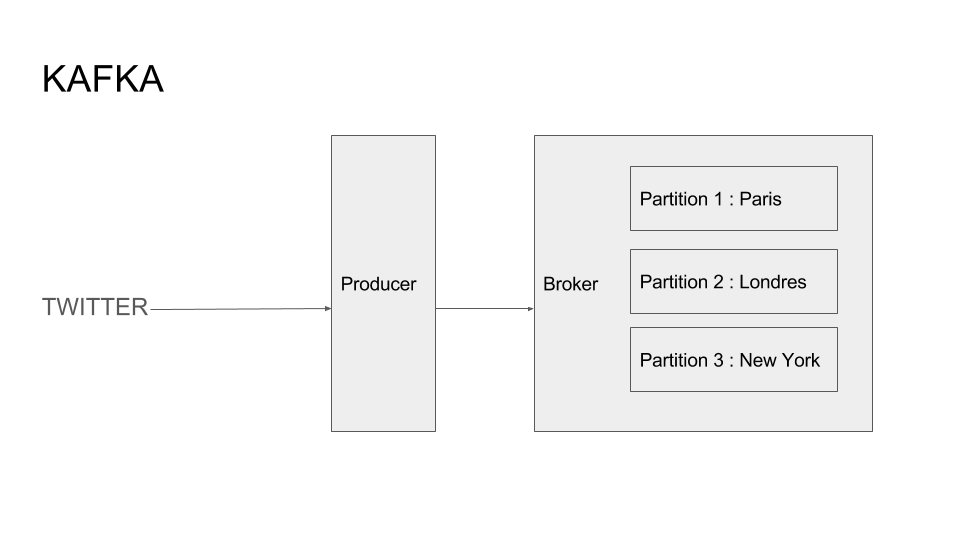
\includegraphics[width=15cm]{content/Kafka.png}
\caption{Kafka est notre premier composant. Nous créons un "Producer" permettant de récupérer le flux de Twitter et filtrant pour récupérer des messages pouvant être lié à la météo. Kafka partitionne ce flux par régions. Seul les régions que nous souhaitons traitées sont gardées}
\label{fig1}
\centering
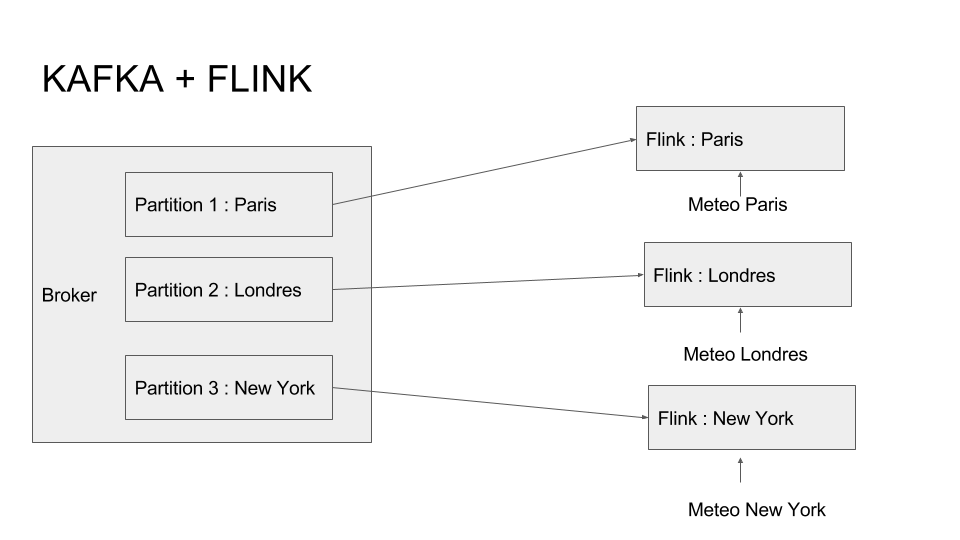
\includegraphics[width=15cm]{content/KafkaFlink.png}
\caption{Flink récupère les données de Kafka correspondant à sa région, traite ces données par rapport aux données météorologiques qu'il à récupéré. Flink récupère les données météorologiques de sa région grâce à une API à intervalles réguliers. }
\label{fig1}
\end{figure}

\pagebreak

\begin{figure}[h]
\centering
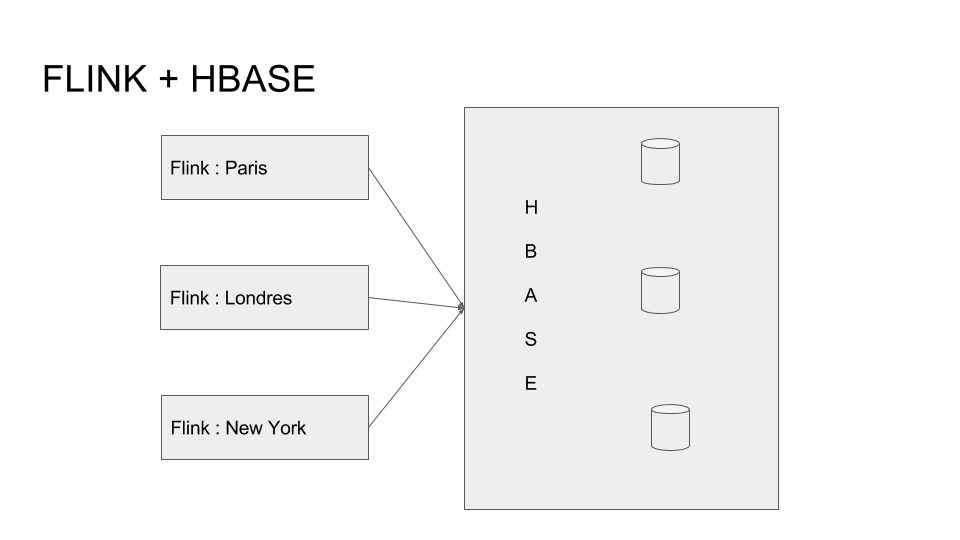
\includegraphics[width=16cm]{content/FlinkHbase.png}
\caption{Lorsque Flink a traité une donnée, il stock son résultat dans la base}
\label{fig1}
\centering
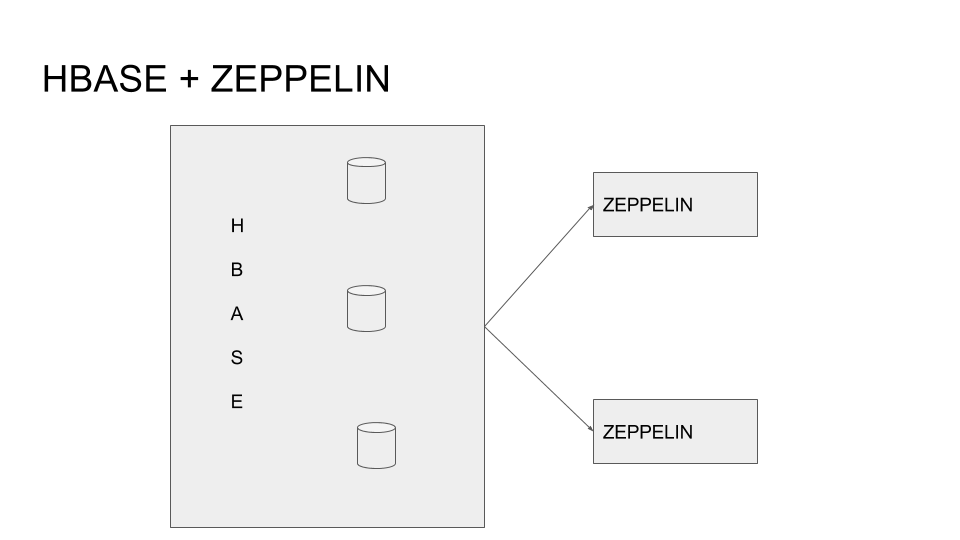
\includegraphics[width=16cm]{content/HbaseZeppelin.png}
\caption{Zeppelin est notre interface de visualisation. Il est connecté à HBase pour récupérer les données}
\label{fig1}
\end{figure}

\pagebreak

\subsection{Premiers objectifs}

\subsubsection{Comportement}

Au départ, nous prenons en compte la présence de 3 serveurs. 
Nous souhaitons garantir le fonctionnement du service en tolérant deux fautes. 

\begin{itemize}
	\item Lorsque 3 machines sont en vie, alors le service fonctionne correctement.
	\item Lorsque 2 machines sont en vie, alors le service fonctionne correctement et cherche à remettre en place la machine en faute.
	\item Lorsque 1 machine est en vie, alors le service fonctionne correctement et à remettre en place les machines en faute. 
\end{itemize}

\subsubsection{Configuration}

\textbf{Kafka}
\begin{itemize}
	\item Installé sur toutes les machines. 
	\item Un détecteur de faute se chargera de détecter les machines fautives.
	\item Un correcteur de faute cherchera à redémarrer la ou les machines fautives
\end{itemize}

\textbf{Flink}
\begin{itemize}
	\item Installé sur 3 machines. 
	\item Un détecteur de faute se chargera de répartir les différentes configurations de Flink sur les différents serveurs en vie
\end{itemize}

\textbf{Hbase}
\begin{itemize}
	\item Installé sur 3 machines. 
\end{itemize}
	
\textbf{Zeppelin}
\begin{itemize}
	\item Installé sur 3 machines. 
	\item Un détecteur de faute cherchera à redémarrer la ou les machines fautives 
\end{itemize}

Nous commencerons par nous fixer un faible nombre de régions (Paris, Londres et New York par exemple). Nous appliquerons nos algorithmes sur ces régions. 
Afin de mesurer le contentement des personnes, nous utiliserons des mots clef, hashtags et emojis contenu dans les messages twitter. 


\subsection{Objectifs suivants}

\subsubsection{Comportement}

Au départ, nous prenons en compte la présence d'un nombre de serveur inconnu par le système mais fixé, appelons le N.

Nous souhaitons garantir le fonctionnement du service(Safe et Live) en tolérant N-2 fautes.
Nous souhaitons garantir le fonctionnement du service(Safe) en tolérant N-1 fautes. 

\begin{itemize}
	\item Lorsque 3 ou plus machines sont en vie, alors le service fonctionne correctement.
	\item Lorsque 2 machines sont en vie, alors le service fonctionne correctement et cherche à remettre en place la machine en faute.
	\item Lorsque 1 machine est en vie, alors le service fonctionne correctement et cherche à remettre en place les machines en faute. 
\end{itemize}


\subsubsection{Configuration}


\textbf{Kafka}
\begin{itemize}
	\item Installé sur 3 machines. 
	\item Un détecteur de faute se chargera de détecter les machines fautives
	\item Un correcteur de faute cherchera à redémarrer la ou les machines fautives
\end{itemize}

\textbf{Flink}
\begin{itemize}
	\item Installé sur $max(3, N-3, N-6, N-9)$ machines. 
	\begin{itemize}
		\item Dans le cas où nous avons de nombreuses régions à traiter, nous évitons de faire tourner Kafka ET Flink sur la meme machine
		\item Il en est de meme pour HBase et Zeppelin
	\end{itemize}
	\item Un détecteur de faute se chargera de répartir les différentes configurations de Flink sur les différents serveurs devant executer Flink
\end{itemize}

\textbf{Hbase}
\begin{itemize}
	\item Installé sur 3 machines. 
\end{itemize}
	
\textbf{Zeppelin}
\begin{itemize}
	\item Installé sur 3 machines. 
\end{itemize}


Avec ces objectifs, nous traiterons un plus grand nombre de régions. 
Afin de mesurer le contentement des personnes, chercherons plus de paramètres à prendre en compte. 



\end{document}
